\documentclass[border=2mm]{standalone}
\usepackage{tikz}
\begin{document}
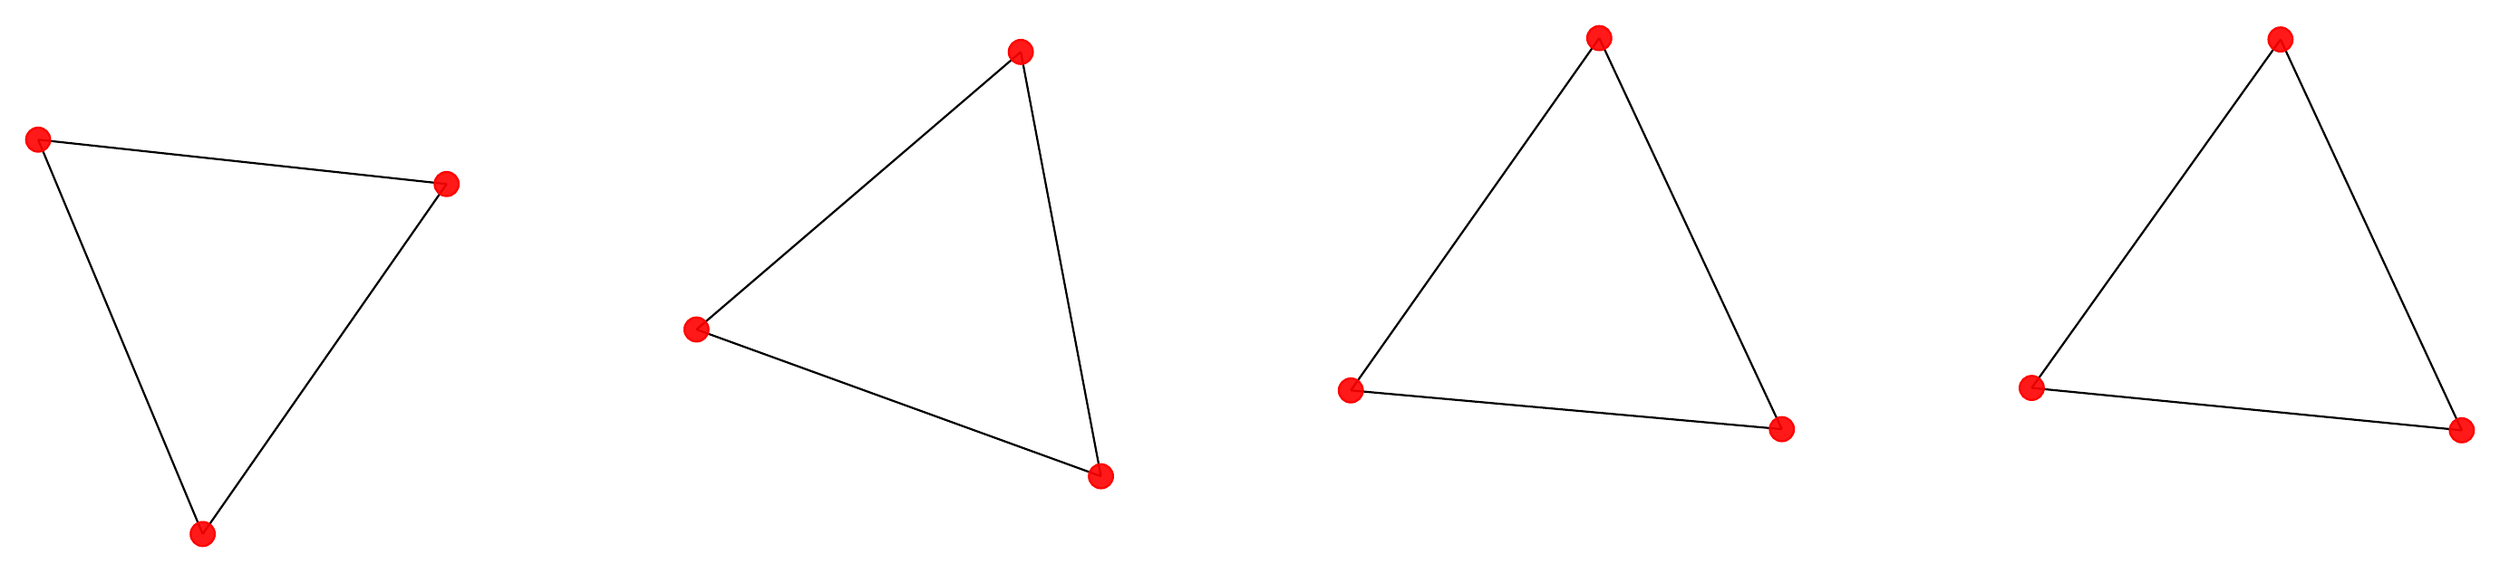
\begin{tikzpicture}[line width=0.5pt,fill opacity=0.9,scale = 3.5]
\tikzstyle{every path}=[draw, thick]
\tikzstyle{every node}=[draw, circle, fill=red, inner sep=3.4pt]
\coordinate (v_0) at (1.65858, -0.99438) {};
\coordinate (v_2) at (1.00000, 0.58607) {};
\coordinate (v_5) at (2.63488, 0.40831) {};
\coordinate (v_1) at (4.93281, 0.93765) {};
\coordinate (v_3) at (5.25362, -0.76290) {};
\coordinate (v_6) at (3.63488, -0.17475) {};
\coordinate (v_4) at (6.25362, -0.41890) {};
\coordinate (v_9) at (7.97887, -0.57423) {};
\coordinate (v_10) at (7.24804, 0.99313) {};
\coordinate (v_7) at (9.97455, 0.98761) {};
\coordinate (v_8) at (8.97887, -0.40894) {};
\coordinate (v_11) at (10.70005, -0.57867) {};
\path (v_0) -- (v_2);
\path (v_0) -- (v_5);
\path (v_1) -- (v_3);
\path (v_1) -- (v_6);
\path (v_2) -- (v_5);
\path (v_3) -- (v_6);
\path (v_4) -- (v_9);
\path (v_4) -- (v_10);
\path (v_7) -- (v_8);
\path (v_7) -- (v_11);
\path (v_8) -- (v_11);
\path (v_9) -- (v_10);
\node[red] (x_0) at (v_0) {};
\node[red] (x_2) at (v_2) {};
\node[red] (x_5) at (v_5) {};
\node[red] (x_1) at (v_1) {};
\node[red] (x_3) at (v_3) {};
\node[red] (x_6) at (v_6) {};
\node[red] (x_4) at (v_4) {};
\node[red] (x_9) at (v_9) {};
\node[red] (x_10) at (v_10) {};
\node[red] (x_7) at (v_7) {};
\node[red] (x_8) at (v_8) {};
\node[red] (x_11) at (v_11) {};
\end{tikzpicture}
\end{document}
